% Options for packages loaded elsewhere
\PassOptionsToPackage{unicode}{hyperref}
\PassOptionsToPackage{hyphens}{url}
\PassOptionsToPackage{dvipsnames,svgnames,x11names}{xcolor}
%
\documentclass[
]{article}

\usepackage{amsmath,amssymb}
\usepackage{iftex}
\ifPDFTeX
  \usepackage[T1]{fontenc}
  \usepackage[utf8]{inputenc}
  \usepackage{textcomp} % provide euro and other symbols
\else % if luatex or xetex
  \usepackage{unicode-math}
  \defaultfontfeatures{Scale=MatchLowercase}
  \defaultfontfeatures[\rmfamily]{Ligatures=TeX,Scale=1}
\fi
\usepackage{lmodern}
\ifPDFTeX\else  
    % xetex/luatex font selection
    \setmainfont[]{Latin Modern Roman}
  \setmathfont[]{Latin Modern Math}
\fi
% Use upquote if available, for straight quotes in verbatim environments
\IfFileExists{upquote.sty}{\usepackage{upquote}}{}
\IfFileExists{microtype.sty}{% use microtype if available
  \usepackage[]{microtype}
  \UseMicrotypeSet[protrusion]{basicmath} % disable protrusion for tt fonts
}{}
\makeatletter
\@ifundefined{KOMAClassName}{% if non-KOMA class
  \IfFileExists{parskip.sty}{%
    \usepackage{parskip}
  }{% else
    \setlength{\parindent}{0pt}
    \setlength{\parskip}{6pt plus 2pt minus 1pt}}
}{% if KOMA class
  \KOMAoptions{parskip=half}}
\makeatother
\usepackage{xcolor}
\setlength{\emergencystretch}{3em} % prevent overfull lines
\setcounter{secnumdepth}{5}
% Make \paragraph and \subparagraph free-standing
\makeatletter
\ifx\paragraph\undefined\else
  \let\oldparagraph\paragraph
  \renewcommand{\paragraph}{
    \@ifstar
      \xxxParagraphStar
      \xxxParagraphNoStar
  }
  \newcommand{\xxxParagraphStar}[1]{\oldparagraph*{#1}\mbox{}}
  \newcommand{\xxxParagraphNoStar}[1]{\oldparagraph{#1}\mbox{}}
\fi
\ifx\subparagraph\undefined\else
  \let\oldsubparagraph\subparagraph
  \renewcommand{\subparagraph}{
    \@ifstar
      \xxxSubParagraphStar
      \xxxSubParagraphNoStar
  }
  \newcommand{\xxxSubParagraphStar}[1]{\oldsubparagraph*{#1}\mbox{}}
  \newcommand{\xxxSubParagraphNoStar}[1]{\oldsubparagraph{#1}\mbox{}}
\fi
\makeatother


\providecommand{\tightlist}{%
  \setlength{\itemsep}{0pt}\setlength{\parskip}{0pt}}\usepackage{longtable,booktabs,array}
\usepackage{calc} % for calculating minipage widths
% Correct order of tables after \paragraph or \subparagraph
\usepackage{etoolbox}
\makeatletter
\patchcmd\longtable{\par}{\if@noskipsec\mbox{}\fi\par}{}{}
\makeatother
% Allow footnotes in longtable head/foot
\IfFileExists{footnotehyper.sty}{\usepackage{footnotehyper}}{\usepackage{footnote}}
\makesavenoteenv{longtable}
\usepackage{graphicx}
\makeatletter
\def\maxwidth{\ifdim\Gin@nat@width>\linewidth\linewidth\else\Gin@nat@width\fi}
\def\maxheight{\ifdim\Gin@nat@height>\textheight\textheight\else\Gin@nat@height\fi}
\makeatother
% Scale images if necessary, so that they will not overflow the page
% margins by default, and it is still possible to overwrite the defaults
% using explicit options in \includegraphics[width, height, ...]{}
\setkeys{Gin}{width=\maxwidth,height=\maxheight,keepaspectratio}
% Set default figure placement to htbp
\makeatletter
\def\fps@figure{htbp}
\makeatother

\usepackage{arxiv}
\usepackage{orcidlink}
\usepackage{amsmath}
\usepackage[T1]{fontenc}
\makeatletter
\@ifpackageloaded{caption}{}{\usepackage{caption}}
\AtBeginDocument{%
\ifdefined\contentsname
  \renewcommand*\contentsname{Table of contents}
\else
  \newcommand\contentsname{Table of contents}
\fi
\ifdefined\listfigurename
  \renewcommand*\listfigurename{List of Figures}
\else
  \newcommand\listfigurename{List of Figures}
\fi
\ifdefined\listtablename
  \renewcommand*\listtablename{List of Tables}
\else
  \newcommand\listtablename{List of Tables}
\fi
\ifdefined\figurename
  \renewcommand*\figurename{Figure}
\else
  \newcommand\figurename{Figure}
\fi
\ifdefined\tablename
  \renewcommand*\tablename{Table}
\else
  \newcommand\tablename{Table}
\fi
}
\@ifpackageloaded{float}{}{\usepackage{float}}
\floatstyle{ruled}
\@ifundefined{c@chapter}{\newfloat{codelisting}{h}{lop}}{\newfloat{codelisting}{h}{lop}[chapter]}
\floatname{codelisting}{Listing}
\newcommand*\listoflistings{\listof{codelisting}{List of Listings}}
\makeatother
\makeatletter
\makeatother
\makeatletter
\@ifpackageloaded{caption}{}{\usepackage{caption}}
\@ifpackageloaded{subcaption}{}{\usepackage{subcaption}}
\makeatother
\makeatletter
\@ifpackageloaded{sidenotes}{}{\usepackage{sidenotes}}
\@ifpackageloaded{marginnote}{}{\usepackage{marginnote}}
\makeatother

\ifLuaTeX
  \usepackage{selnolig}  % disable illegal ligatures
\fi
\usepackage{bookmark}

\IfFileExists{xurl.sty}{\usepackage{xurl}}{} % add URL line breaks if available
\urlstyle{same} % disable monospaced font for URLs
\hypersetup{
  pdftitle={Experiment Result: Two Phase Flow},
  pdfauthor={Jayjay, Tuna, Jason, Richard},
  colorlinks=true,
  linkcolor={blue},
  filecolor={Maroon},
  citecolor={Blue},
  urlcolor={Blue},
  pdfcreator={LaTeX via pandoc}}


\renewcommand{\today}{2024-09-30}
\newcommand{\runninghead}{A Preprint }
\renewcommand{\runninghead}{A Preprint }
\title{Experiment Result: Two Phase Flow}
\def\asep{\\\\\\ } % default: all authors on same column
\author{\textbf{Jayjay, Tuna, Jason, Richard}\\}
\date{2024-09-30}
\begin{document}
\maketitle


\section{Updates}\label{updates}

\begin{enumerate}
\def\labelenumi{\arabic{enumi}.}
\tightlist
\item
  \textbf{Debugged inference method}
\item
  \textbf{With the updated inference method, did hyperparameter search,
  especially with learning rate, \(\lambda\)}
\item
  We were wondering why it seemed like there was not so much
  improvement.
\item
  \textbf{We retrained the model with updated eigenvector}
  -\textgreater{} refer to Updated Experiment Setting
\item
  Loss decreases faster, posterior
\end{enumerate}

\section{Previous Experiment Setting}\label{previous-experiment-setting}

\begin{enumerate}
\def\labelenumi{\arabic{enumi}.}
\tightlist
\item
  \textbf{Dataset}

  \begin{itemize}
  \tightlist
  \item
    \(2000\) pairs of \(\{K, S^t(K)\}_{t=1}^8\).
  \item
    Train Test split: {[}1800, 200{]}
  \end{itemize}
\item
  \textbf{FIM}

  \begin{itemize}
  \tightlist
  \item
    Number of observation = 10
  \item
    Number of eigenvector = 1
  \item
    For a single pair of datapoint, we obtain 1 FIM.

    \begin{itemize}
    \tightlist
    \item
      Likelihood is difference between perturbed time series of
      \(\{S^t(K)\}_{t=1}^8\) with true time series of
      \(\{S^t(K)\}_{t=1}^8\).
    \end{itemize}
  \end{itemize}
\item
  \textbf{Hyperparameter}

  \begin{itemize}
  \tightlist
  \item
    Batchsize = 100
  \end{itemize}
\end{enumerate}

\section{Updated Experiment Setting}\label{updated-experiment-setting}

\begin{enumerate}
\def\labelenumi{\arabic{enumi}.}
\tightlist
\item
  \textbf{Dataset}

  \begin{itemize}
  \tightlist
  \item
    \(1000\) pairs of \(\{K, S^t(K)\}_{t=1}^8\).
  \item
    Train Test split: {[}800, 200{]}
  \end{itemize}
\item
  \textbf{FIM}

  \begin{itemize}
  \tightlist
  \item
    Number of observation = 2
  \item
    Number of eigenvector = 1
  \item
    For a single pair of datapoint, we obtain 8 FIM as there are 8
    different time steps.

    \begin{itemize}
    \tightlist
    \item
      Likelihood is difference between perturbed single Saturation
      \(S^t(K)\) with true singe time step Saturation.
    \end{itemize}
  \end{itemize}
\item
  \textbf{Hyperparameter}

  \begin{itemize}
  \tightlist
  \item
    Batchsize = 100
  \end{itemize}
\end{enumerate}

\section{Pipeline}\label{pipeline}

\begin{itemize}
\tightlist
\item
  \textbf{FNO-NF.jl}: create two-phase flow dataset, eigenvector of FIM,
  and vJp
\item
  \textbf{Diff\_MultiPhysics}: train (written in pytorch) and posterior
  estimation
\end{itemize}

\section{Training Result}\label{training-result}

To evaluate training result, we go over three things:

\begin{itemize}
\tightlist
\item
  Loss Behavior
\item
  Forward Simulation
\item
  Posterior Estimation
\end{itemize}

\subsection{Loss/Learning Behavior}\label{losslearning-behavior}

\begin{figure}

\begin{minipage}{0.50\linewidth}

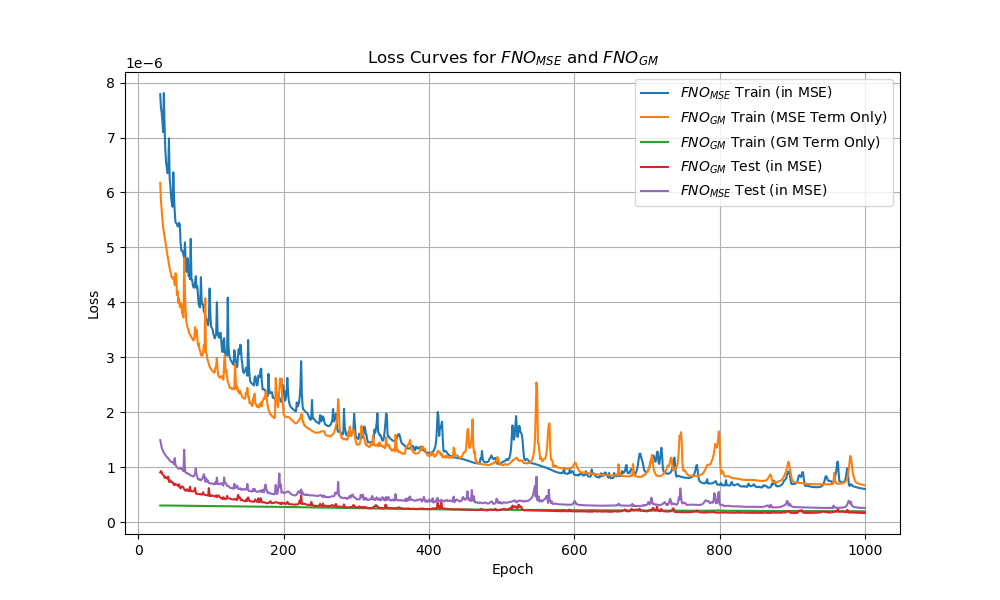
\includegraphics[width=1\textwidth,height=\textheight]{../../test/all_loss.png}

\subcaption{\label{}All loss}
\end{minipage}%
%
\begin{minipage}{0.50\linewidth}

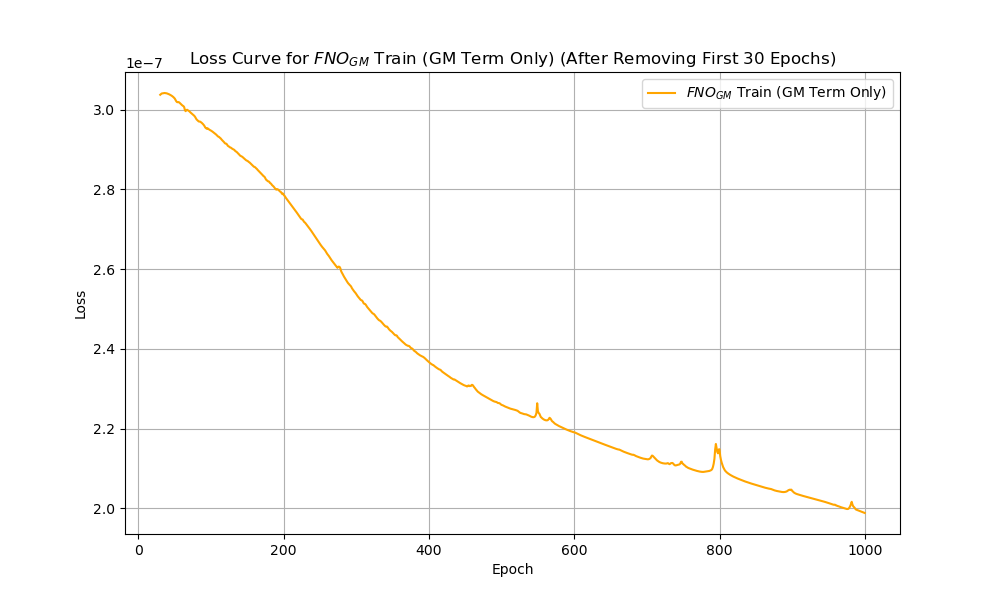
\includegraphics[width=1\textwidth,height=\textheight]{../../test/GM_term.png}

\subcaption{\label{}Only GM Term}
\end{minipage}%

\caption{\label{fig-loss}Example Loss plots (GM model:3rd row of the
loss table)}

\end{figure}%

\begin{longtable}[]{@{}
  >{\raggedright\arraybackslash}p{(\columnwidth - 8\tabcolsep) * \real{0.1852}}
  >{\raggedright\arraybackslash}p{(\columnwidth - 8\tabcolsep) * \real{0.1111}}
  >{\raggedright\arraybackslash}p{(\columnwidth - 8\tabcolsep) * \real{0.1111}}
  >{\raggedright\arraybackslash}p{(\columnwidth - 8\tabcolsep) * \real{0.2963}}
  >{\raggedright\arraybackslash}p{(\columnwidth - 8\tabcolsep) * \real{0.2963}}@{}}
\toprule\noalign{}
\begin{minipage}[b]{\linewidth}\raggedright
\end{minipage} & \begin{minipage}[b]{\linewidth}\raggedright
Epochs
\end{minipage} & \begin{minipage}[b]{\linewidth}\raggedright
\(\lambda\)
\end{minipage} & \begin{minipage}[b]{\linewidth}\raggedright
Train Loss
\end{minipage} & \begin{minipage}[b]{\linewidth}\raggedright
Test Loss
\end{minipage} \\
\midrule\noalign{}
\endhead
\bottomrule\noalign{}
\endlastfoot
& & & MSE/GM & MSE \\
FNO-MSE & 1000 & N.A. & \(3.3622 \times 10^{-8}\) &
\textbf{\(8.4016 \times 10^{-8}\)} \\
FNO-PBI & 2000 & 150.0 & \(1.0436 \times 10^{-7}\) &
\(1.044 \times 10^{-7}\) \\
FNO-PBI & 2000 & 1.0 & \(3.0028 \times 10^{-8}\) &
\(8.0099 \times 10^{-8}\) \\
FNO-PBI & 1000 & 150.0 & \(2.6428 \times 10^{-7}\) &
\(1.5976 \times 10^{-7}\) \\
FNO-PBI & 1000 & 20.0 & \(6.2106 \times 10^{-8}\) &
\(9.2973 \times 10^{-8}\) \\
FNO-PBI & 1000 & 5.0 & \(6.3265 \times 10^{-8}\) &
\(9.7524 \times 10^{-8}\) \\
FNO-PBI & 1000 & 1.0 & \(4.1154 \times 10^{-8}\) &
\textbf{\(8.6791 \times 10^{-8}\)} \\
FNO-PBI & 1000 & 0.7 & \(4.2235 \times 10^{-8}\) &
\(9.1102 \times 10^{-8}\) \\
\end{longtable}

Updated loss table

\begin{longtable}[]{@{}
  >{\raggedright\arraybackslash}p{(\columnwidth - 8\tabcolsep) * \real{0.1852}}
  >{\raggedright\arraybackslash}p{(\columnwidth - 8\tabcolsep) * \real{0.1111}}
  >{\raggedright\arraybackslash}p{(\columnwidth - 8\tabcolsep) * \real{0.1111}}
  >{\raggedright\arraybackslash}p{(\columnwidth - 8\tabcolsep) * \real{0.2963}}
  >{\raggedright\arraybackslash}p{(\columnwidth - 8\tabcolsep) * \real{0.2963}}@{}}
\toprule\noalign{}
\begin{minipage}[b]{\linewidth}\raggedright
\end{minipage} & \begin{minipage}[b]{\linewidth}\raggedright
Epochs
\end{minipage} & \begin{minipage}[b]{\linewidth}\raggedright
\(\lambda\)
\end{minipage} & \begin{minipage}[b]{\linewidth}\raggedright
Train Loss
\end{minipage} & \begin{minipage}[b]{\linewidth}\raggedright
Test Loss
\end{minipage} \\
\midrule\noalign{}
\endhead
\bottomrule\noalign{}
\endlastfoot
& & & MSE/GM & MSE \\
FNO-MSE & 1000 & 1.0 & \(6.5207 \times 10^{-8}\) &
\(1.3088 \times 10^{-7}\) \\
FNO-PBI & 1000 & 1.0 & \(8.3925 \times 10^{-8}\) &
\(1.3030\times 10^{-7}\) \\
\end{longtable}

We now evaluate surrogate models in two different criteria, forward
simulation and inverse problem.

\subsection{Evaluation: Forward
Simulation}\label{evaluation-forward-simulation}

\subsubsection{Forward Simulation on test
sample}\label{forward-simulation-on-test-sample}

\begin{figure}

\begin{minipage}{\linewidth}

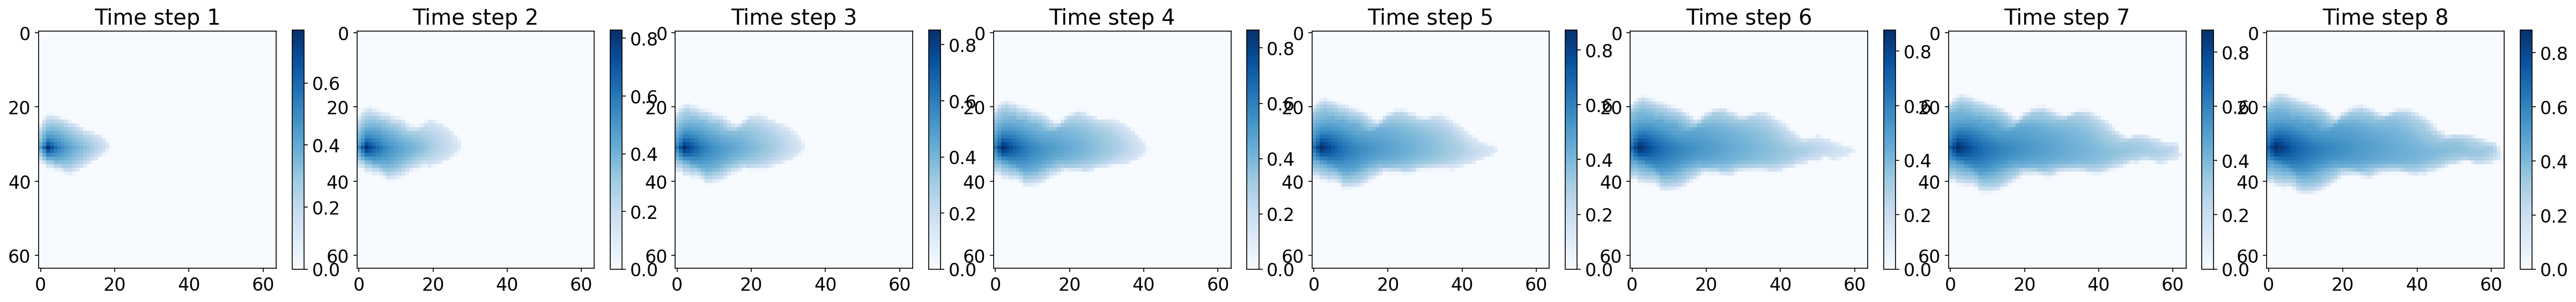
\includegraphics[width=1\textwidth,height=\textheight]{../../plot/GCS_channel_plot/FNO_GCS_lowest_MSE_True.png}

\subcaption{\label{}True Saturation}
\end{minipage}%
\newline
\begin{minipage}{\linewidth}

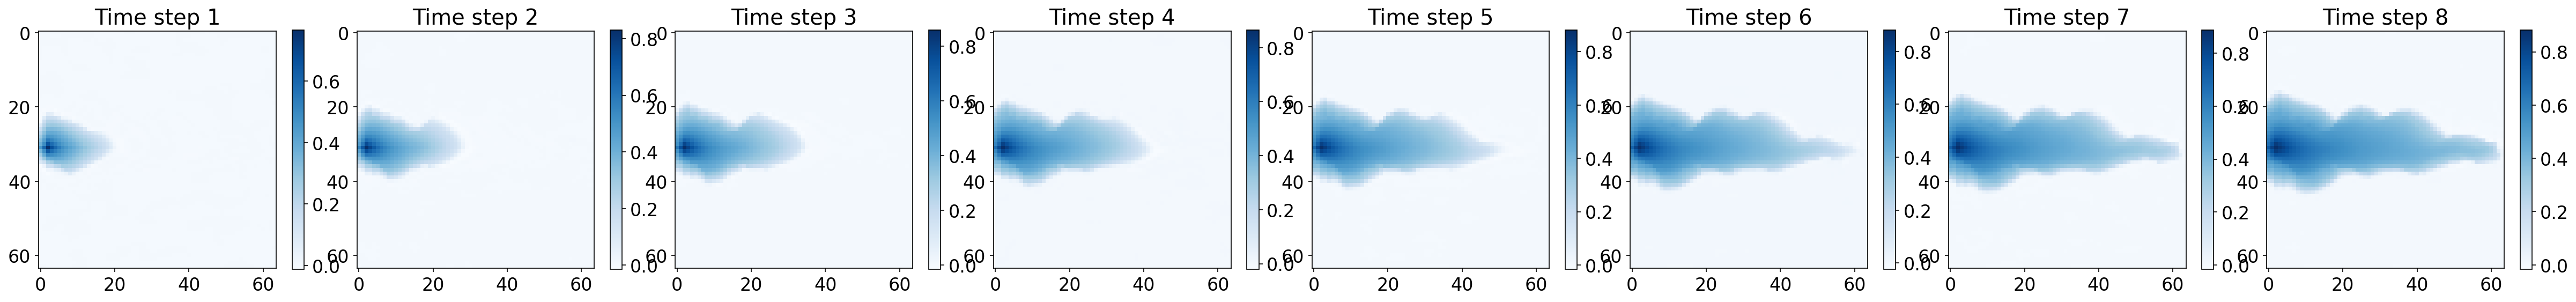
\includegraphics[width=1\textwidth,height=\textheight]{../../plot/GCS_channel_plot/FNO_GCS_lowest_MSE_Pred.png}

\subcaption{\label{}Predicted Saturation: MSE}
\end{minipage}%
\newline
\begin{minipage}{\linewidth}

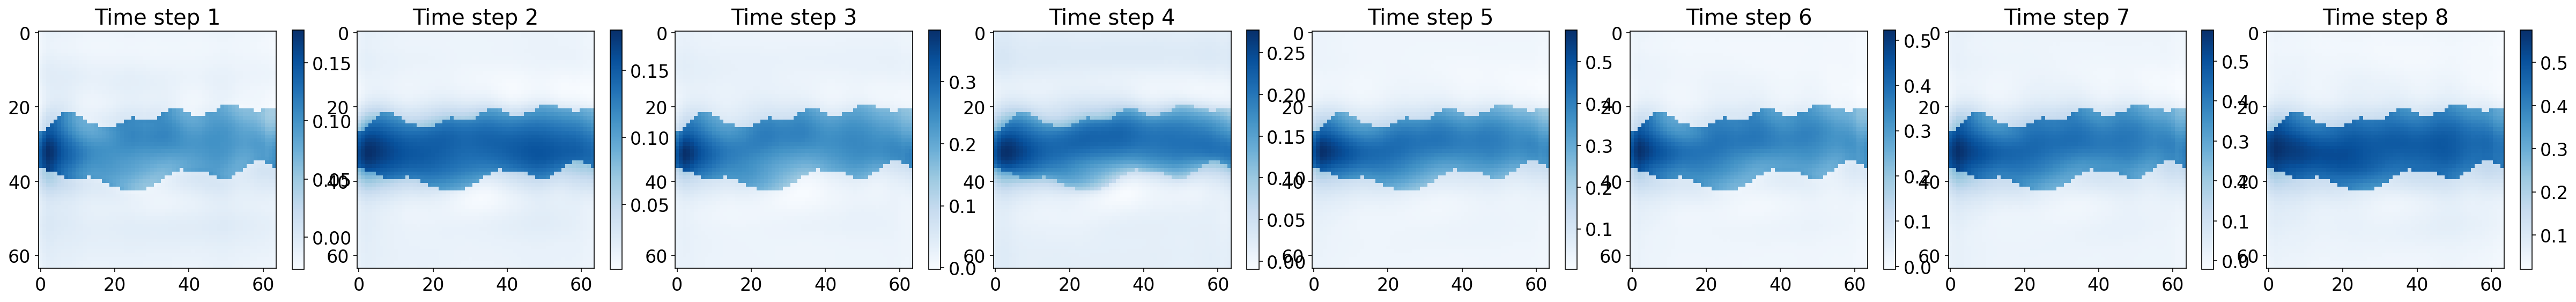
\includegraphics[width=1\textwidth,height=\textheight]{../../plot/GCS_channel_plot/FNO_GCS_lowest_JAC_Pred.png}

\subcaption{\label{}Predicted Saturation: PBI}
\end{minipage}%

\caption{\label{fig-eig1000}Example of Forward Prediction}

\end{figure}%

\begin{figure}

\begin{minipage}{\linewidth}

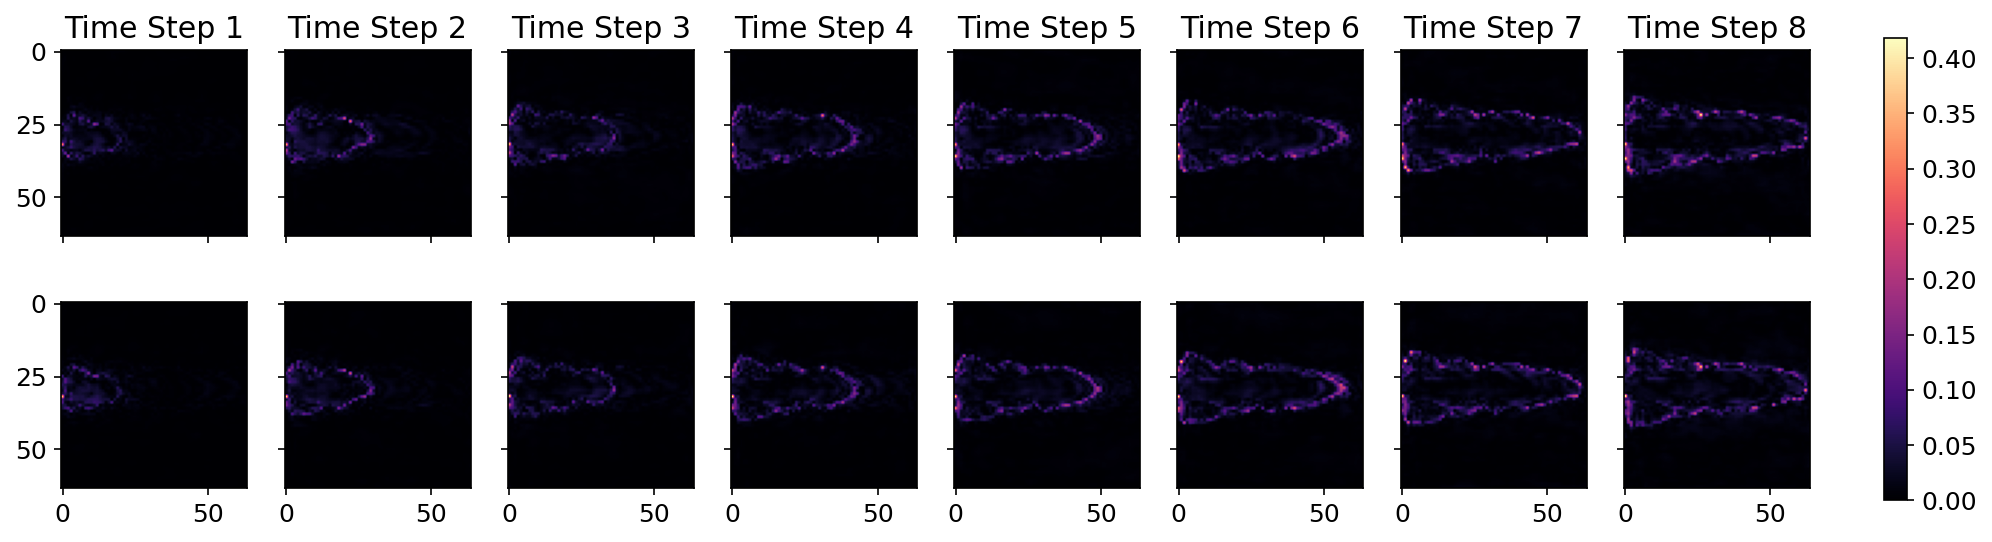
\includegraphics[width=1\textwidth,height=\textheight]{../../gen_sample/GCS_sample/forward_pred_test_diff1.png}

\subcaption{\label{}Test Sample 1}
\end{minipage}%
\newline
\begin{minipage}{\linewidth}

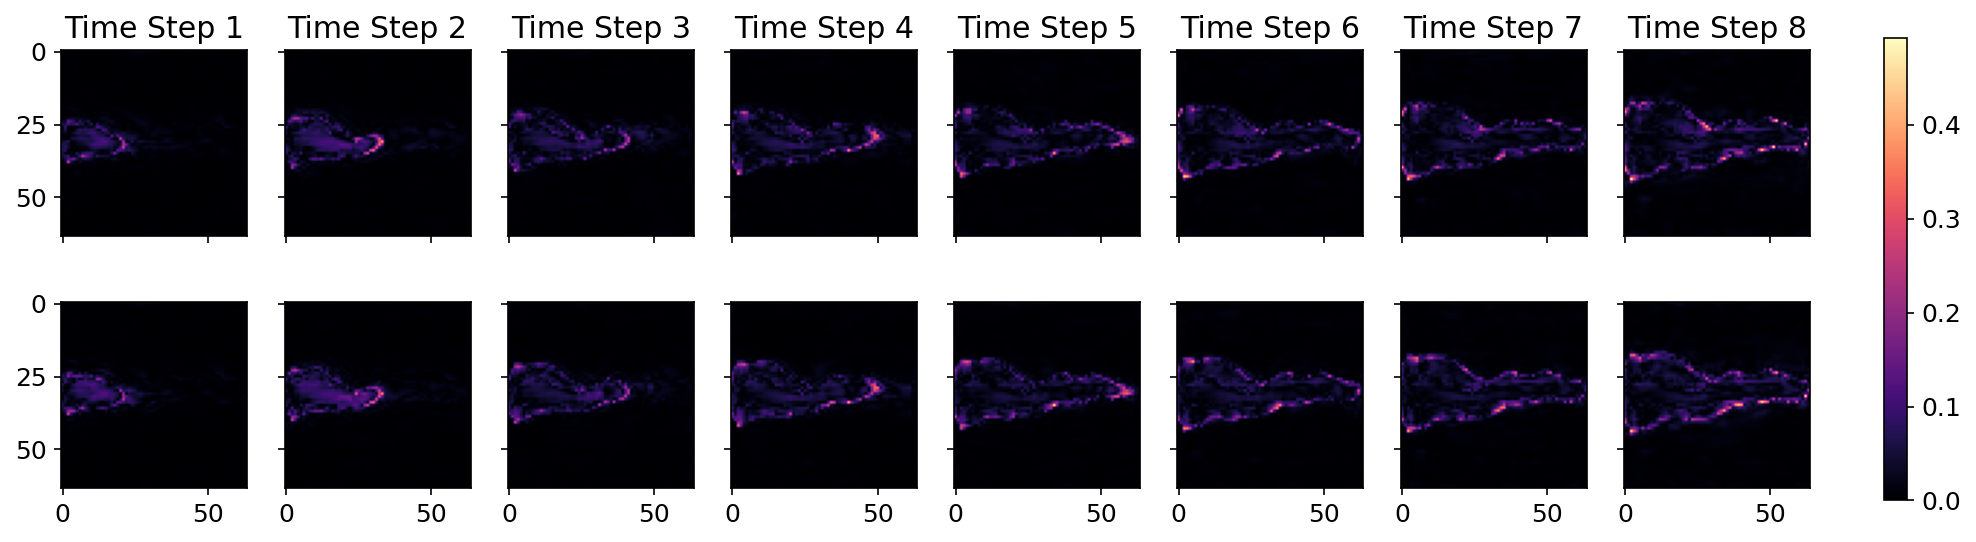
\includegraphics[width=1\textwidth,height=\textheight]{../../gen_sample/GCS_sample/forward_pred_test_diff2.png}

\subcaption{\label{}Test Sample 2}
\end{minipage}%
\newline
\begin{minipage}{\linewidth}

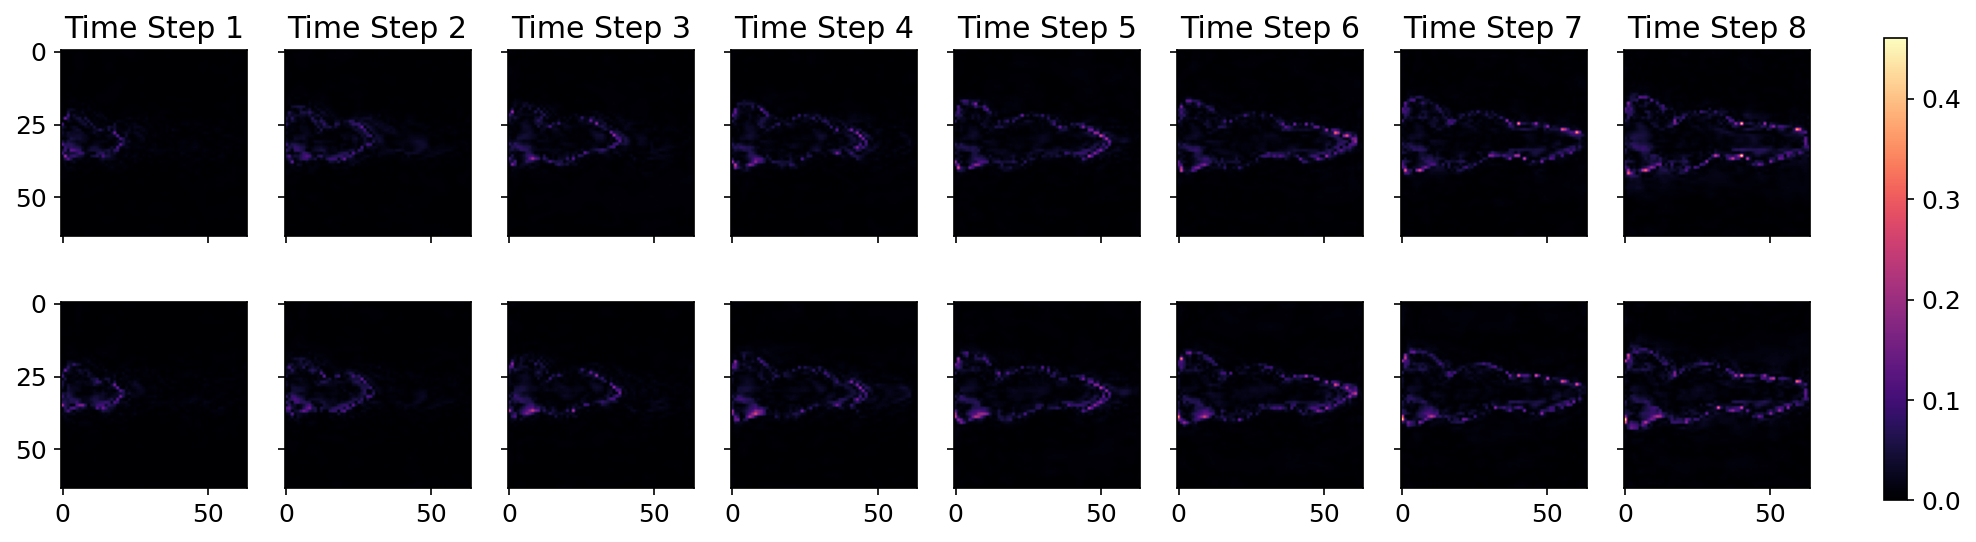
\includegraphics[width=1\textwidth,height=\textheight]{../../gen_sample/GCS_sample/forward_pred_test_diff3.png}

\subcaption{\label{}Test Sample 3}
\end{minipage}%

\caption{\label{fig-eig1000}Absolute Difference plot of test samples}

\end{figure}%

\subsubsection{Learned and True vjp (sanity
check)}\label{learned-and-true-vjp-sanity-check}

We observe that for MSE,

\begin{enumerate}
\def\labelenumi{\arabic{enumi}.}
\tightlist
\item
  Scale in the color bar does not match.
\item
  The learned vjp looks noisy as there are some colors showing in the
  part where it should be just white.
\end{enumerate}

But in PBI, we verify that the learned vjp and true vjp matches well.

\begin{enumerate}
\def\labelenumi{\arabic{enumi}.}
\tightlist
\item
  The scale of color bar matches correctly.
\item
  The plot does not look noisy.
\end{enumerate}

\begin{figure}[H]

{\centering 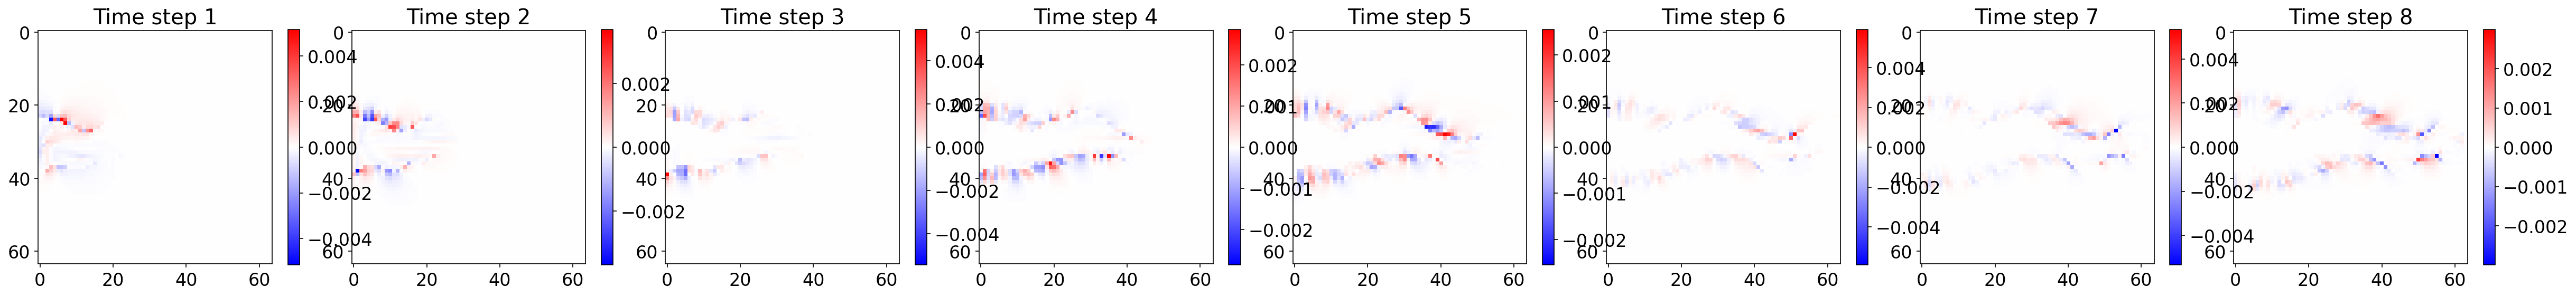
\includegraphics[width=1\textwidth,height=\textheight]{../../plot/GCS_channel_plot/training/MSE/true_vjp_1.png}

}

\caption{True vjp}

\end{figure}%%
\begin{figure}[H]

{\centering 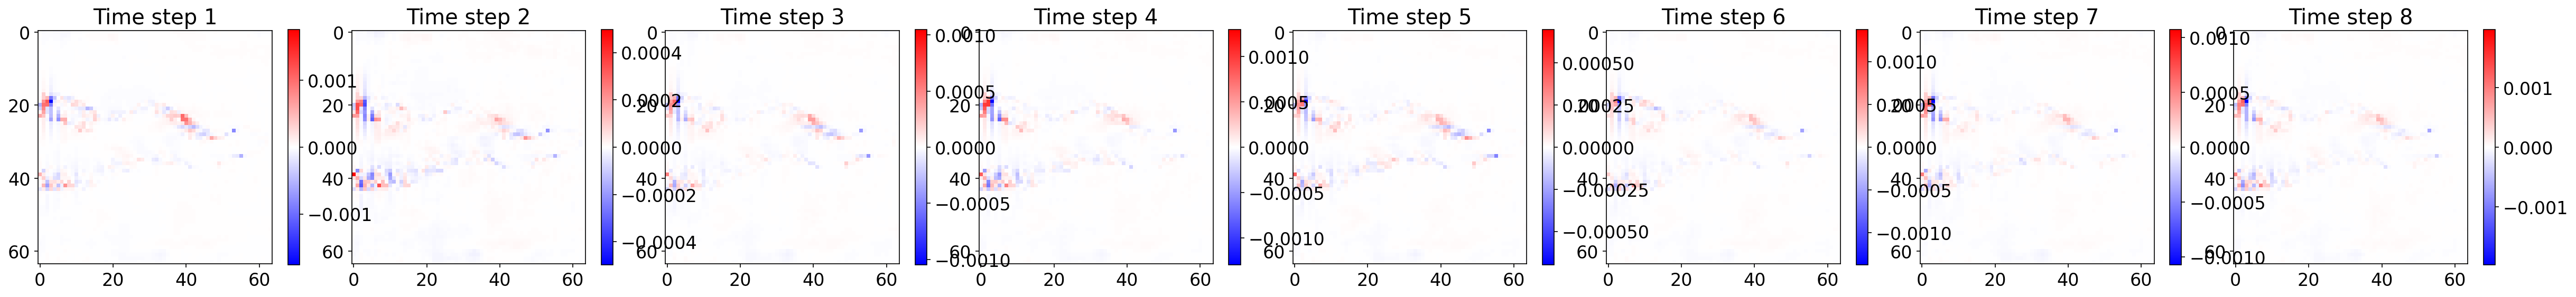
\includegraphics[width=1\textwidth,height=\textheight]{../../plot/GCS_channel_plot/training/MSE/learned_vjp_990.png}

}

\caption{Learned vjp: MSE}

\end{figure}%%
\begin{figure}[H]

{\centering 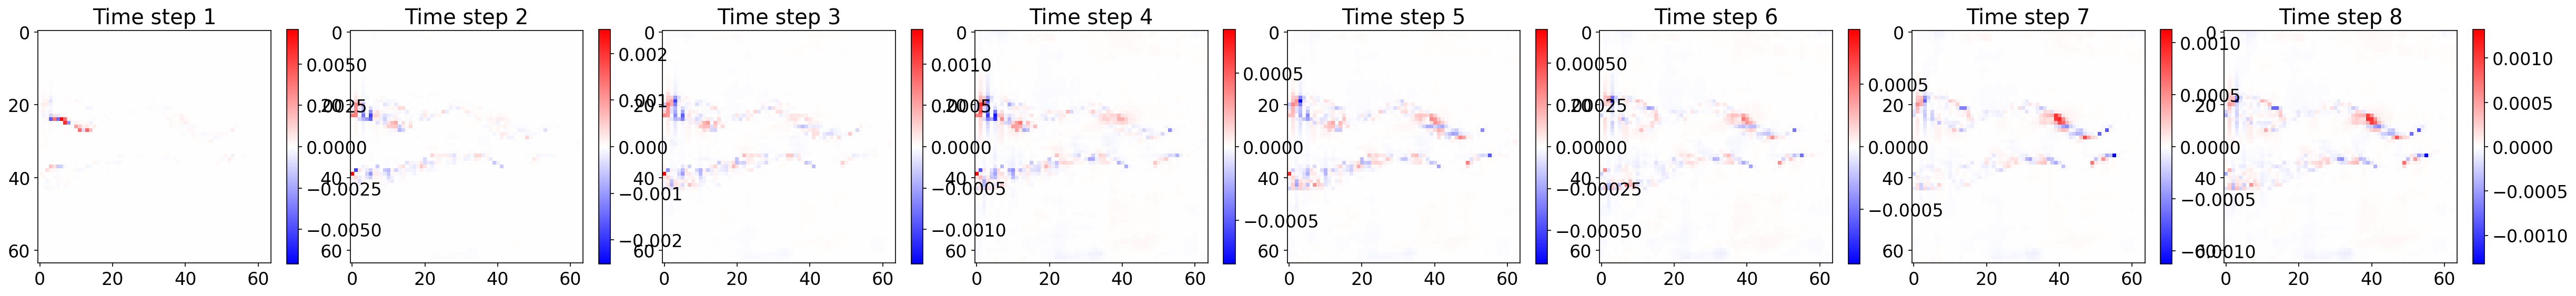
\includegraphics[width=1\textwidth,height=\textheight]{../../plot/GCS_channel_plot/training/JAC/learned_vjp_990.png}

}

\caption{Learned vjp: PBI}

\end{figure}%%
\begin{figure}[H]

{\centering 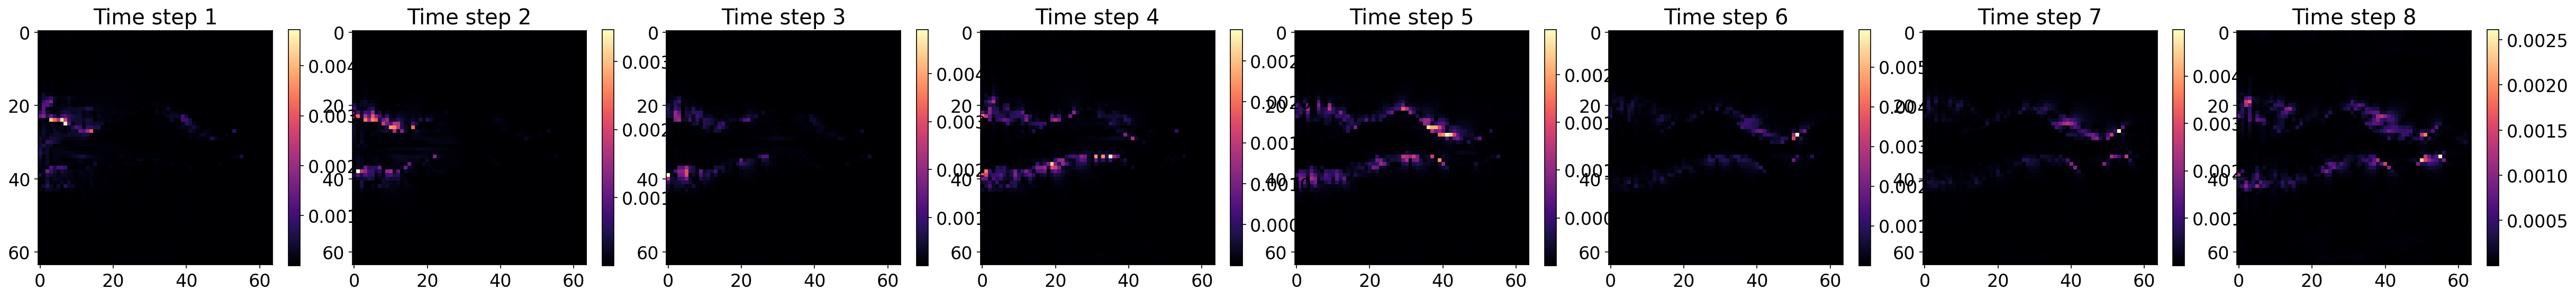
\includegraphics[width=1\textwidth,height=\textheight]{../../plot/GCS_channel_plot/training/MSE/diff_vjp_990.png}

}

\caption{Absolute Difference: MSE}

\end{figure}%%
\begin{figure}[H]

{\centering 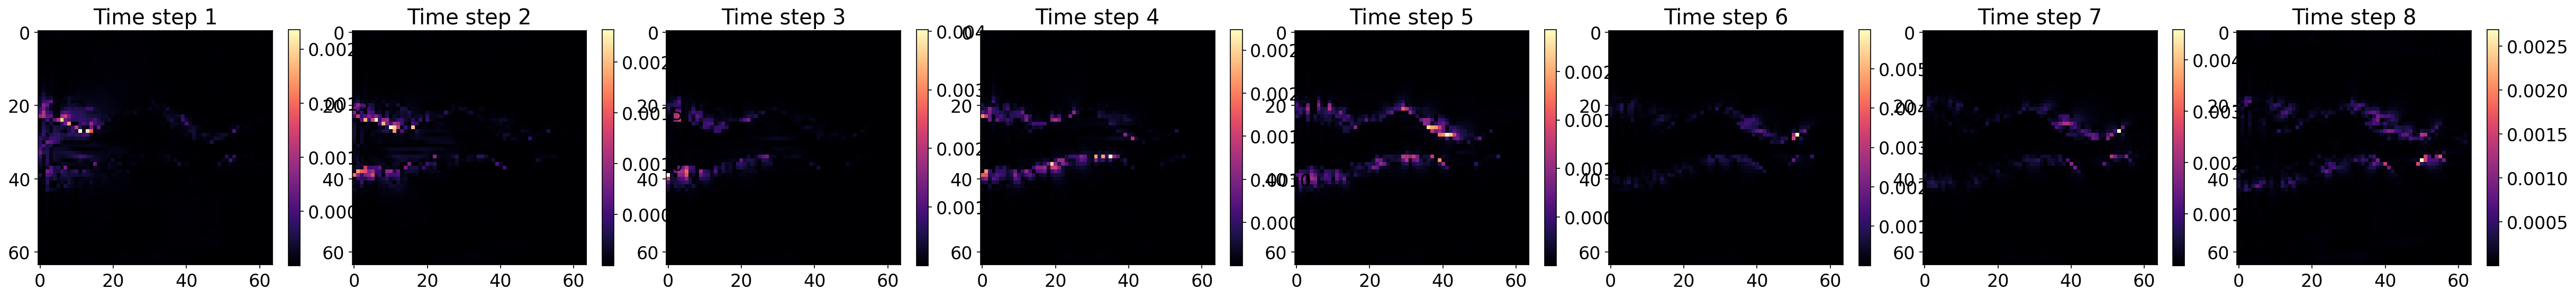
\includegraphics[width=1\textwidth,height=\textheight]{../../plot/GCS_channel_plot/training/JAC/diff_vjp_990.png}

}

\caption{Absolute Difference: PBI}

\end{figure}%

\subsubsection{What other things can be evaluated in terms of forward
simulation?}\label{what-other-things-can-be-evaluated-in-terms-of-forward-simulation}

\begin{enumerate}
\def\labelenumi{\arabic{enumi}.}
\tightlist
\item
  \textbf{Stability}: predict longer saturation evolution 9th to 16th.
\item
  \textbf{Generalization}: test with out of distribution test samples.
\end{enumerate}

\subsubsection{Toy example to test generalizability of MSE and
PBI}\label{toy-example-to-test-generalizability-of-mse-and-pbi}

Also, generated \textbf{out of distribution samples}:

\begin{figure}

\begin{minipage}{0.50\linewidth}

\includegraphics[width=0.8\textwidth,height=\textheight]{../../data/ood_K_1.png}

\subcaption{\label{}out of distribution: K}
\end{minipage}%
%
\begin{minipage}{0.50\linewidth}

\centering{

\includegraphics[width=0.8\textwidth,height=\textheight]{../../data/Ks_0.png}

}

\subcaption{\label{fig-surus}In distribution K}

\end{minipage}%

\caption{\label{fig-K}In distribution K and out of distribution K}

\end{figure}%

\begin{figure}[H]

{\centering \includegraphics[width=1\textwidth,height=\textheight]{../../data/ood_S_1.png}

}

\caption{OOD: S}

\end{figure}%%
\begin{figure}[H]

{\centering 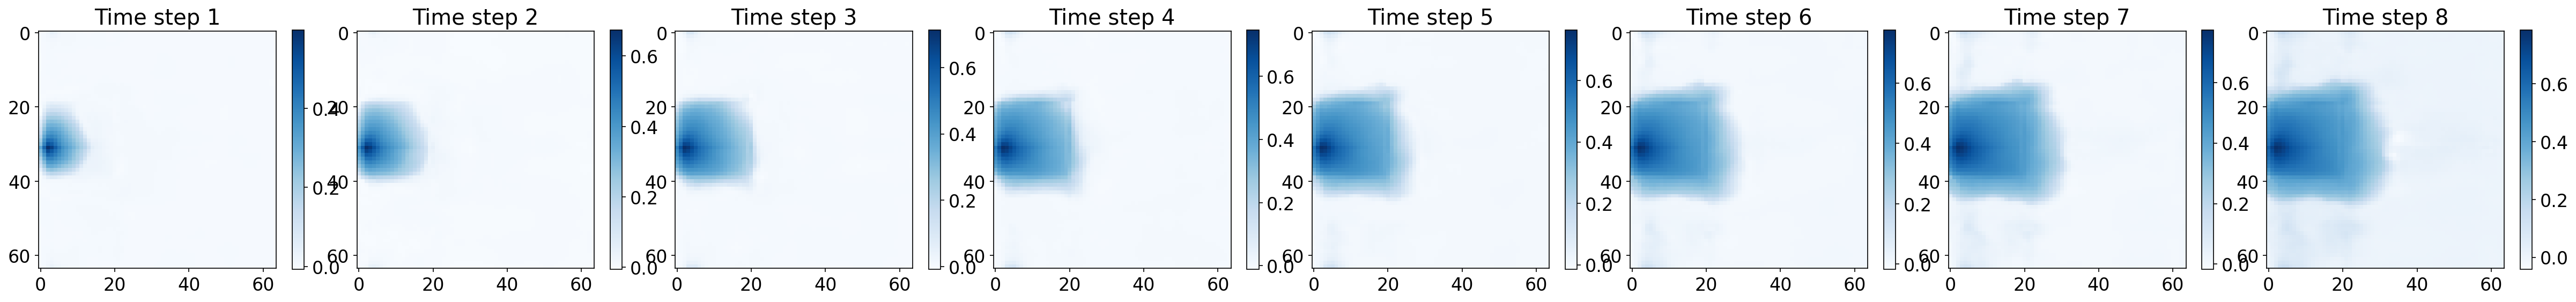
\includegraphics[width=1\textwidth,height=\textheight]{../../gen_sample/GCS_sample/ood_mse_1.png}

}

\caption{OOD: MSE Forward Prediction}

\end{figure}%%
\begin{figure}[H]

{\centering 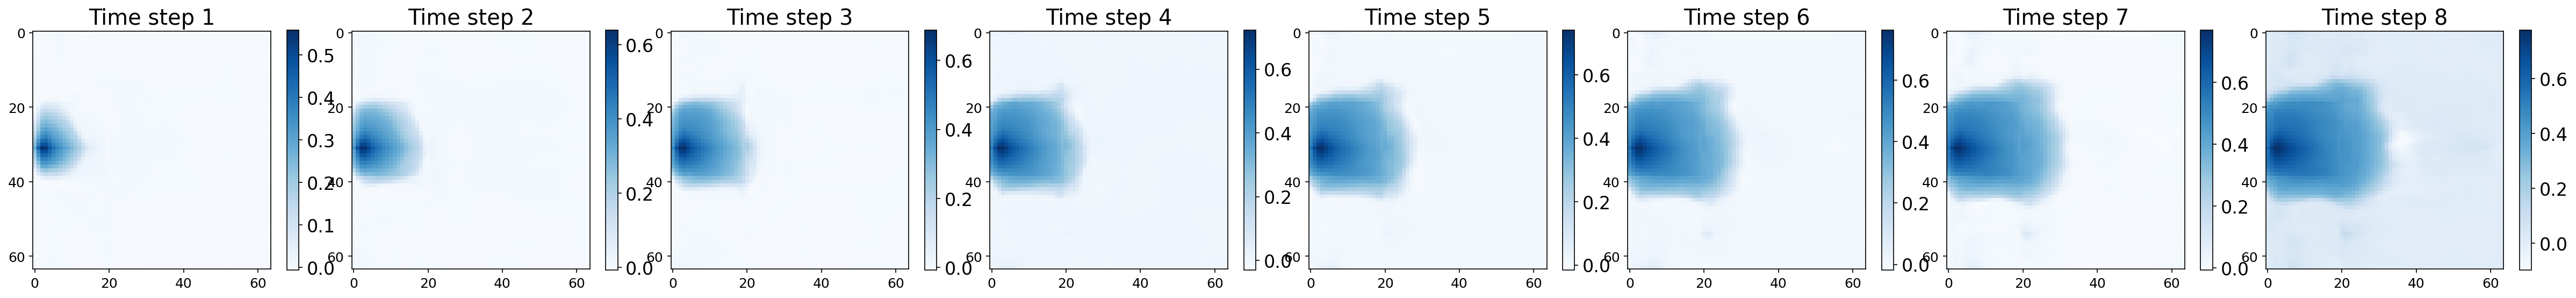
\includegraphics[width=1\textwidth,height=\textheight]{../../gen_sample/GCS_sample/ood_jac_1.png}

}

\caption{OOD: PBI Forward Prediction}

\end{figure}%%
\begin{figure}[H]

{\centering 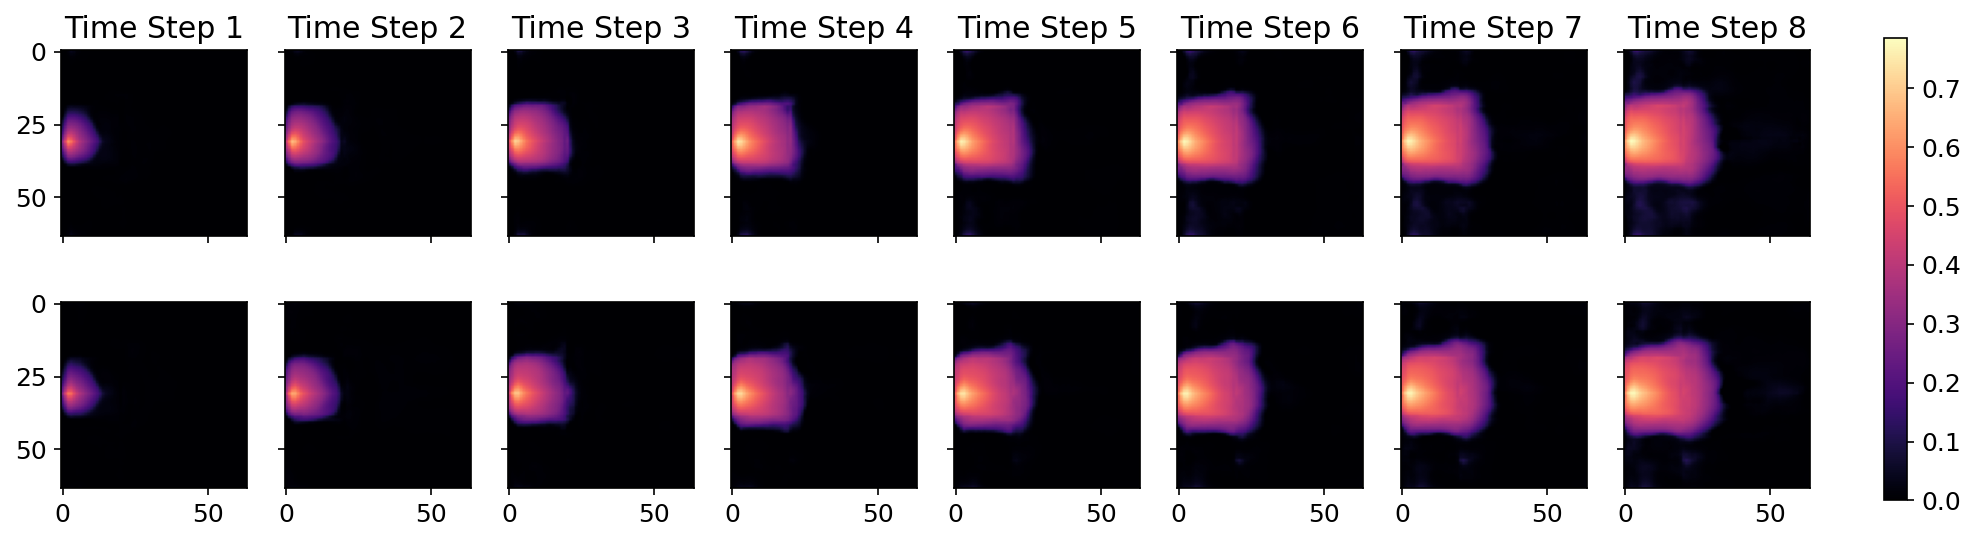
\includegraphics[width=1\textwidth,height=\textheight]{../../gen_sample/GCS_sample/ood_diff_1.png}

}

\caption{OOD: diff btw learned posterior and K}

\end{figure}%

\subsubsection{Things to change in experiment for better forward
prediction of
PBI}\label{things-to-change-in-experiment-for-better-forward-prediction-of-pbi}

But before conducting all those experiments, we might want to change the
eigenvector. That is,

\begin{itemize}
\item
  From single eigenvector for single datapair,\(\{K, S^t(K)\}_{t=1}^8\),
  we generate eight different eigenvector to better inform time dynamics
  of plume.
\item
  Currently, the number of observation is 10. Increase to 100.
\end{itemize}

\subsection{Evaluation: Posterior
Estimate}\label{evaluation-posterior-estimate}

\[ min_{K} \|S_{\theta}(K) - S(K*) \|^2_2 \]

where: - K0 = H(K) - S\_\{\theta\}: Neural Network model

\subsubsection{Choosing the best parameters for MLE
optimization}\label{choosing-the-best-parameters-for-mle-optimization}

We conduct hyperparameter search for the \(\lambda\). The number of
epochs chosen were based on the loss plot convergence. If it converged,
we stopped training.

This is unconstrained. When lambda = 1., it is not accurate.

\paragraph{Unconstrained}\label{unconstrained}

\begin{longtable}[]{@{}
  >{\raggedright\arraybackslash}p{(\columnwidth - 8\tabcolsep) * \real{0.2055}}
  >{\raggedright\arraybackslash}p{(\columnwidth - 8\tabcolsep) * \real{0.1233}}
  >{\raggedright\arraybackslash}p{(\columnwidth - 8\tabcolsep) * \real{0.1233}}
  >{\raggedright\arraybackslash}p{(\columnwidth - 8\tabcolsep) * \real{0.3288}}
  >{\raggedright\arraybackslash}p{(\columnwidth - 8\tabcolsep) * \real{0.2192}}@{}}
\toprule\noalign{}
\begin{minipage}[b]{\linewidth}\raggedright
\end{minipage} & \begin{minipage}[b]{\linewidth}\raggedright
Epochs
\end{minipage} & \begin{minipage}[b]{\linewidth}\raggedright
\(\lambda\)
\end{minipage} & \begin{minipage}[b]{\linewidth}\raggedright
Loss (MSE)
\end{minipage} & \begin{minipage}[b]{\linewidth}\raggedright
SSIM
\end{minipage} \\
\midrule\noalign{}
\endhead
\bottomrule\noalign{}
\endlastfoot
FNO-PBI & 800 & 1.0 & \(4.2823 \times 10^{-4}\) & \(63.8013\) \\
FNO-PBI & 400 & 20.0 & \(8.9021 \times 10^{-5}\) & \(55.5040\) \\
FNO-PBI & 300 & 50.0 & \(6.1867 \times 10^{-5}\) & \(55.5502\) \\
FNO-PBI & 200 & 100.0 & \(5.5757 \times 10^{-5}\) & \(57.0893\) \\
--------------- & --------- & --------- & ------------------------ &
---------------- \\
FNO-MSE & 800 & 1.0 & \(3.0692 \times 10^{-4}\) & \(57.3091\) \\
FNO-MSE & 400 & 20.0 & \(5.3901 \times 10^{-5}\) & \(52.3515\) \\
FNO-MSE & 300 & 50.0 & \(3.4602 \times 10^{-5}\) & \(54.2848\) \\
FNO-MSE & 200 & 100.0 & \(2.9429 \times 10^{-5}\) & \(55.6442\) \\
\end{longtable}

\subsubsection{Updated Result}\label{updated-result}

Originally, we wanted to use Normalizing Flow for our inference method.
But because it takes quite a long time to train, for a quick evaluation,
we first try least squares method. Out of all 200 test samples, I
brought some interesting cases.

\begin{figure}[H]

{\centering \includegraphics[width=1\textwidth,height=\textheight]{../../gen_sample/GCS_partial/both_0_200/posterior_400_0_23.png}

}

\caption{Test sample 1}

\end{figure}%%
\begin{figure}[H]

{\centering \includegraphics[width=1\textwidth,height=\textheight]{../../gen_sample/GCS_partial/both_0_200/posterior_400_0_24.png}

}

\caption{Test sample 2}

\end{figure}%%
\begin{figure}[H]

{\centering \includegraphics[width=1\textwidth,height=\textheight]{../../gen_sample/GCS_partial/both_0_200/posterior_400_0_25.png}

}

\caption{Test sample 3}

\end{figure}%%
\begin{figure}[H]

{\centering \includegraphics[width=1\textwidth,height=\textheight]{../../gen_sample/GCS_partial/both_0_200/posterior_400_0_26.png}

}

\caption{Test sample 4}

\end{figure}%%
\begin{figure}[H]

{\centering \includegraphics[width=1\textwidth,height=\textheight]{../../gen_sample/GCS_partial/both_0_200/posterior_400_0_27.png}

}

\caption{Test sample 5}

\end{figure}%

\section{Conclusion}\label{conclusion}

\begin{itemize}
\tightlist
\item
  As of right now, we don't see significant difference between MSE and
  PBI model in terms of posterior estimate.

  \begin{itemize}
  \tightlist
  \item
    It is likely undertrained.
  \end{itemize}
\end{itemize}

\subsection{Future Step}\label{future-step}

\begin{enumerate}
\def\labelenumi{\arabic{enumi}.}
\tightlist
\item
  TODO: Debug NS eigenvector and vjp.
\item
  TODO: Want to generate the full dataset for Francis' dataset (which
  might take 1 or 2 days).
\item
  TODO: Try it on Jason's dataset (Now that we fixed the problem with
  FIM computation, we are optimistic about the experiment, so we want to
  try it again.)
\end{enumerate}

\subsection{Question}\label{question}

\begin{enumerate}
\def\labelenumi{\arabic{enumi}.}
\tightlist
\item
  Do we want to train both models for a longer time?
\end{enumerate}




\end{document}
